\documentclass[12pt,a4paper,openright,twoside]{book}
\usepackage[utf8]{inputenc}
\usepackage{amsmath}
\usepackage{amssymb}
\usepackage{listings}
\usepackage{algorithm}
\usepackage{algpseudocode}
\usepackage{tabularx}
\usepackage{graphics}
\usepackage{disi-thesis}
\usepackage{code-lstlistings}
\usepackage{notes}
\usepackage{shortcuts}
\usepackage{acronym}
%\usepackage[linesnumbered,ruled,vlined]{algorithm2e}


\newcommand{\thesislang}{english} % commentare in caso di tesi in italiano
%\usepackage{thesis-style}
% version
%\newcommand{\versionmajor}{0}
%\newcommand{\versionminor}{1}
%\newcommand{\versionpatch}{2}
%\newcommand{\version}{\versionmajor.\versionminor.\versionpatch}
%\typeout{Document version: \version}

\school{\unibo}
\programme{Corso di Laurea Magistrale in Ingegneria e Scienze Informatiche}
\title{Fair-by-design algoriths for access to education}
\author{Antonio Iannotta}
\date{\today}
\subject{Intelligent Systems Engineering}
\supervisor{Prof. Giovanni Ciatto}
\cosupervisor{Prof. Roberta Calegari}
\morecosupervisor{Prof. Andrea Omicini}
\session{IV}
\academicyear{2022-2023}

% Definition of acronyms
\acrodef{IoT}{Internet of Thing}
\acrodef{vm}[VM]{Virtual Machine}
\acrodef{AI}{Artificial Intelligence}


\mainlinespacing{1.241} % line spacing in mainmatter, comment to default

\begin{document}
	
\frontmatter

% ! TeX root = thesis-main.tex
\title{Title}
\author{Candidate Name Here}
\date{\today}

\newgeometry{margin=0.8in}
\begin{titlepage}
	\begin{center}
		% \vspace*{0.2cm}
		
		\large
		\textbf{ALMA MATER STUDIORUM -- UNIVERSITÀ DI BOLOGNA \\ CAMPUS DI CESENA}
		\\
		\noindent\hrulefill
		\vspace{0.4cm}
		
		\Large
		Scuola di Ingegneria e Architettura \\
		Corso di Laurea Magistrale in Ingegneria e Scienze Informatiche
		
		\Huge
		\vspace{4cm}
		\textbf{
			Fair-by-design algorithm for access to education
		}
		
		\large
		\vspace{1cm}
		Tesi di laurea in 
		\\
		\textsc{Intelligent System Engineering}
		
		\vspace{5.5cm}
		\begin{minipage}[t]{0.64\textwidth}
			\begin{flushleft}
				\textit{Relatore} 
				\\ 
				\textbf{Prof.} \textbf{Giovanni Ciatto}
				\\
				\vspace{0.4cm}
				\textit{Correlatore} 
				\\
				\textbf{Prof.} \textbf{Roberta Calegari}
				\textbf{Prof.} \textbf{Andre Omicini}
			\end{flushleft}
		\end{minipage}
		\begin{minipage}[t]{0.34\textwidth}
			\begin{flushright}
				\textit{Candidato} 
				\\ 
				\textbf{Antonio Iannotta}
			\end{flushright}
		\end{minipage}\\
		
		\vfill
		\noindent\hrulefill
		\vspace{0.3cm}
		\Large
		
		IV Sessione di Laurea
		\\
		Anno Accademico 2022-2023
	\end{center}
\end{titlepage}
\restoregeometry


\begin{abstract}

    This work presents an in-depth approach to address fairness and bias mitigation in the design and development of data-driven methods. The primary contribution of this study is the proposal and implementation of an innovative \emph{Fair-by-Design} workflow that incorporates various strategies for bias mitigation within data, algorithms, and decision-making processes.

    The work focuses on the educational data of the Canary Islands, leveraging a dataset encompassing detailed information about student performance and educational outcomes.

    The primary objective is to ensure equitable and unbiased application of data-driven algorithms within the educational context. 

    The methodology involves the systematic evaluation of multiple bias mitigation strategies. The critical aspect of this research centers on the comparison of these strategies based on their impact on the predictive accuracy of the algorithms. 

    This approach provides practical insights into the trade-offs between fairness and accuracy, showing how several approaches can lead to different accuracy scores on the same dataset and with the same models. 

    The work findings offer valuable insights into the trade-offs between fairness and accuracy when developing data-driven methods for educational data. 

    This thesis contributes to the ongoing discourse on fairness in machine learning and data-driven decision-making. The results provide guidance for stakeholders in the education sector, aiding them in making informed decisions about algorithm deployment to promote fairness and minimize bias within educational systems. 

\end{abstract}
    


%\begin{acknowledgements} % this is optional
%Never too far down, to come back
%\end{acknowledgements}

%----------------------------------------------------------------------------------------
\tableofcontents   
%\listoffigures     % (optional) comment if empty
%\lstlistoflistings % (optional) comment if empty
%----------------------------------------------------------------------------------------

\mainmatter

%----------------------------------------------------------------------------------------
\chapter{Introduction}
\label{chap:introduction}
%----------------------------------------------------------------------------------------

Artificial Intelligence (AI) has experienced an unprecedented surge in prominence and utility in recent years, emerging as a transformative force across diverse domains. From powering autonomous vehicles to aiding healthcare diagnosis and recommendation systems, AI applications have become increasingly woven into the fabric of our daily lives. However, this rapid proliferation has ushered in a pressing concern about the pervasive presence of bias within AI systems.

The concept of bias in AI pertains to the inadvertent or systematic preference shown towards specific groups or characteristics within the data, algorithms, or decision-making processes. This partiality leads to outcomes that are unjust, unfair, and unequal. In this era of AI-driven decision-making, the imperative to address bias is not just a technological challenge but a moral and societal necessity. Additionally, the ethical principle of fairness underscores the collective aspiration to ensure that AI systems yield equitable and just results for all individuals, regardless of their personal attributes.

The repercussions of bias and unfairness in AI systems extend far beyond mere technological concerns. These issues carry profound societal implications, impacting vital areas such as employment, education, and access to critical services. Biased AI systems perpetuate and exacerbate existing inequalities, inadvertently reinforcing harmful stereotypes and undermining the foundational principles of justice and equality.

In the realm of education, data-driven decision-making has gained significant ground, with educational institutions increasingly relying on AI systems for tasks ranging from student admissions to evaluating learning outcomes and allocating educational resources. The stakes in this domain are notably high. Ensuring that these AI-driven education systems mitigate bias and prioritize fairness is not just a technological endeavor; it is a moral and societal imperative.

The Fair-by-Design workflow presented extends the traditional machine learning workflow by explicitly incorporating fairness considerations from the outset of AI system design. This approach aims to proactively address and mitigate bias throughout the development process, ensuring fairness is not an afterthought but an integral part of the system's foundation.

This work proposes the Fair-by-Design workflow, offering multiple solutions to address fairness challenges within AI systems. We explore and implement three distinct approaches within this workflow, each contributing to the overarching goal of fostering fairness in AI.

The objective is to compare not only the accuracy but also the value of specific fairness metrics at the conclusion of the workflow. By contrasting these outcomes with a scenario where fairness assumptions are not made, we aim to provide a comprehensive assessment of both accuracy and fairness within the proposed framework.

The structure of this thesis unfolds as follows: The \cref{chap:background} conducts a thorough review of the existing approaches and methodologies designed to address bias and promote fairness in the development of AI systems. This chapter lays the groundwork upon which our innovative Fair-by-Design workflow is built. The \cref{chap:contribution} chapter delves into the intricacies of the workflow, elucidating the seamless integration of various fairness approaches into the design process. The \cref{chap:validation} meticulously presents the results derived from the application of these fairness approaches, offering an empirical comparison of their performance and effectiveness. Finally, the \cref{chap:conclusions} not only imparts insights gleaned from our research but also outlines prospective directions for further advancements in this critical and ever-evolving field.

%----------------------------------------------------------------------------------------
\chapter{State of the Art} % or Background
\label{chap:background}

This chapter provides a comprehensive overview of the preceding works and the scientific literature that have paved the way for the implementation of fair-by-design methods in our research. The journey begins with a thorough examination of the multifaceted field of \emph{artificial intelligence} and its wide-ranging applications, including its pivotal roles in critical sectors and socio-technical systems. Within this context, we delve deeply into the intricate issues of \emph{bias} and \emph{fairness} in AI systems, acknowledging the essential foundation upon which our work is built. 

Artificial Intelligence (\emph{AI}) stands at the forefront of technological innovation, significantly reshaping diverse sectors, from healthcare to finance and transportation. To comprehensively grasp the transformative potential of AI, it is essential to explore its applications and the complex ecosystems in which it operates. This chapter endeavors to unravel the intricate web of AI systems and their profound impact on society.

However, the proliferation of AI brings with it the inherent challenge of bias. As AI systems learn from vast datasets, they may inadvertently perpetuate and exacerbate existing prejudices, resulting in \emph{bias} within the algorithms. Recognizing this challenge as a critical one, our exploration extends into the various dimensions of bias, highlighting its multifaceted nature and the potential consequences it carries. 

Moreover, in our quest for equitable AI, the concept of \emph{fairness} emerges as a beacon of hope. This chapter dissects the concept of fairness within AI systems, exploring the intricate ethical considerations that underlie the pursuit of equitable outcomes for all individuals. The chapter further investigates technical dimensions of fairness, acknowledging that it is not merely a goal but a fundamental ethical principle that underpins our work. 

Through this comprehensive exploration, we pave the way for the implementation of fair-by-design methods. This chapter is not only a testament to the foundation on which our research stands but also a testament to the complexity of the AI landscape, its potential for societal transformation, and the imperative of mitigating bias and promoting fairness as we forge ahead in the development of AI systems. 


\section{Artificial Intelligence}

This chapter embarks on a deep dive into the dynamic and multifaceted realm of Artificial Intelligence (AI) and Machine Learning (ML), two groundbreaking technologies that are reshaping human interaction with the world. AI, as a vast and encompassing domain, denotes the development of computer systems endowed with the capability to perform tasks traditionally reserved for human intelligence. These tasks span the spectrum from speech recognition to intricate problem-solving and adaptive learning. 

Within the expansive domain of AI, Machine Learning emerges as a prominent subset, taking center stage in this exploration. Machine Learning is a field that focuses on creating algorithms that empower computers to discern intricate patterns within data and make informed predictions. At its core, Machine Learning excels at enhancing performance over time by processing and assimilating data. The essence of Machine Learning lies in its ability to autonomously learn from data, continuously adapting and improving its decision-making capabilities. 

The AI and ML landscape encompasses a diverse array of techniques and methodologies. Notable examples include Natural Language Processing, Computer Vision, Robotics, and Expert Systems, each wielding distinct capabilities and applications. Machine Learning, in particular, is a repository of algorithms crafted to enable machines to self-learn and refine their performance sans explicit programming. These algorithms grant machines the ability to make data-driven decisions, essentially automating the process of pattern recognition and prediction. 

The transformative impact of AI extends far beyond the horizon, with direct implications for critical sectors, including healthcare and autonomous driving, where the consequences are not merely abstract but can be a matter of life and death. However, the profound influence of AI is not confined to these sectors alone. It permeates socio-technical systems, which are emblematic of the intricate interplay between individuals, technology, and social institutions. 

Socio-technical systems are marked by the intricate interplay between individuals, technology, and social institutions. AI and ML have catalyzed substantial transformations within these systems, profoundly altering how individuals interact with technology and reshaping the fabric of society. As AI becomes increasingly embedded in the social fabric, it is imperative to confront the intricate ethical quandaries it raises. 

The integration of AI and ML within these systems has precipitated a cascade of intricate ethical dilemmas. These encompass concerns surrounding data privacy, the pervasive presence of biases inherent in algorithms, and the impending potential for job displacement due to automation. In this context, constructing robust ethical frameworks is not just a matter of academic discourse but an essential imperative. 

These ethical frameworks serve as a safeguard, ensuring that AI systems adhere to the principles of fairness, transparency, and accountability. They stand as the bulwark against potential harm and serve to distribute the benefits of AI equitably across society. As this chapter unfolds, it endeavors to delve deeper into these ethical considerations, offering insights into how technology and ethics converge in the evolving landscape of AI and ML. \cite{GRUETZEMACHER2022102884}.

\newpage
\section{Traditional Machine Learning Workflow}

The traditional machine learning (ML) workflow comprises several fundamental steps, each playing a crucial role in the development of predictive models. These steps are designed to transform raw data into a trained and evaluated model. The following sections outline the four main stages of the traditional ML workflow: data acquisition, data pre-processing, modeling, and performance evaluation.

\subsection{Data Acquisition}

The first step in any machine learning project is acquiring the necessary data. This involves identifying and collecting datasets relevant to the problem at hand. The quality and quantity of the data directly impact the performance and generalization ability of the model. Data acquisition may involve obtaining datasets from public repositories, creating custom datasets, or integrating data from various sources.

\subsection{Data Pre-processing}

Once the data is collected, it undergoes pre-processing to make it suitable for training machine learning models. This stage involves cleaning the data to handle missing values, removing outliers, and addressing any inconsistencies. Additionally, feature engineering may be performed to extract relevant information and create new features. Data normalization or scaling may also be applied to ensure that all features contribute equally to the model.

\subsection{Modeling}

With pre-processed data, the next step is to select and train a machine learning model. This involves choosing an appropriate algorithm based on the nature of the problem (classification, regression, etc.) and the characteristics of the data. The selected model is then trained on a portion of the dataset, learning the patterns and relationships within the data. Hyperparameter tuning may be conducted to optimize the model's performance.

\subsection{Performance Evaluation}

The final stage of the traditional ML workflow is evaluating the model's performance on unseen data. This is typically done using a separate test dataset that the model has not encountered during training. Common evaluation metrics include accuracy, precision, recall, F1 score, and area under the receiver operating characteristic (ROC) curve. The goal is to assess how well the model generalizes to new, unseen instances and to identify areas for potential improvement.

\newpage
\section{Bias}

Artificial Intelligence (AI) is undeniably a transformative force, poised to reshape multiple dimensions of our existence in profound ways. Its versatile applications extend far and wide, from refining and expediting decision-making processes to seamlessly automating mundane and repetitive tasks. In this ever-evolving landscape, AI systems are becoming increasingly integrated into our daily experiences, orchestrating a paradigm shift in how we interact with the world around us. 

However, amidst the excitement and optimism surrounding AI's potential, a growing concern resonates both within the AI community and society as a whole. This concern revolves around the pervasive issue of biases intricately woven into the very fabric of AI algorithms. 

These biases, often unintentional and subtle, can seep into AI systems through the data they are trained on and the methods employed to develop them. As AI systems learn from historical data, they may inadvertently inherit the prejudices and stereotypes present in those datasets. Consequently, these biases can manifest in various ways, perpetuating and amplifying societal inequalities. For example, in AI applications for hiring or lending, biases can result in unfair discrimination based on factors such as race or gender. In automated content recommendations, biases can reinforce echo chambers, limiting exposure to diverse perspectives and ideas. 

The consequences of these biases are far-reaching and profound. They not only undermine the ethical foundations of AI but can also erode trust in these technologies. As AI systems gain prominence in critical areas like healthcare, criminal justice, and education, the ramifications of bias become increasingly worrisome. 

Addressing bias in AI is a complex and ongoing challenge. It requires a multifaceted approach that encompasses not only improved data collection and curation but also transparency in AI decision-making processes. Researchers and engineers are working tirelessly to develop techniques for bias detection and mitigation. Additionally, there is a growing push for diverse representation in the AI development community to ensure that the creation of AI systems considers a wide array of perspectives. 

In conclusion, while the promise of AI is immense, the journey towards harnessing its potential responsibly and equitably is an imperative one. As we move forward in this AI-driven era, it is essential to remain vigilant in identifying and rectifying biases, ensuring that AI truly serves as a force for positive change in our evolving world. \cite{10.1145/3308560.3317590}

\subsection{Understanding Bias in AI}

Bias in AI is a critical issue, signifying the presence of unjust and skewed representations or treatment of individuals or groups based on attributes such as race, gender, age, socioeconomic status, or other defining characteristics. These biases are deeply embedded in AI systems and can persist throughout their development and training processes. They arise from a variety of sources, including historical data imbalances, deeply ingrained societal prejudices, and imperfections in the algorithms themselves.

\subsection{Sources of Bias}

\subsubsection{Historical data} 

The issue of bias originating from historical data is a critical and intricate challenge that looms large in the landscape of machine learning. When machine learning models are trained on datasets culled from the annals of history, they inevitably inherit the biases and patterns encoded within that data. These historical biases, often a reflection of deeply ingrained societal prejudices and structural inequalities, can persist and intensify when the model is operationalized. \cite{10.1145/3308560.3317590}

Consider a scenario where historical data contains systemic biases against specific demographics, such as gender, race, or other socio-demographic attributes. The machine learning model, in its quest to optimize performance, dutifully replicates and perpetuates these biases in its predictions and decision-making processes. The consequence of this perpetuation is the perpetuation of historical injustices, potentially leading to the endorsement of discriminatory practices and the exacerbation of preexisting societal inequalities, significantly disadvantaging certain groups. 

Effectively addressing bias originating from historical data necessitates a multidimensional approach, coupled with proactive measures. The first step involves diligent data preprocessing techniques aimed at the identification and subsequent mitigation of bias-laden elements within the dataset. These techniques span a spectrum from data re-sampling to re-weighting and data augmentation, designed to restore balance and fairness. 

Simultaneously, interventions in algorithmic fairness are introduced to the machine learning process. These interventions encompass a range of techniques, including re-weighting of training instances, the introduction of fairness constraints, and adversarial debiasing methods, all aimed at guiding the model toward making fair and equitable predictions. 

Moreover, the journey toward equitable AI is an ongoing one, requiring constant vigilance. Continuous monitoring and adjustment of models, often in real-time, become imperative to ensure that fairness is upheld and biased outcomes are identified and rectified. 

Ultimately, the overarching goal is to foster a future where machine learning not only learns from historical data but actively works to transcend the bonds of bias. In this vision, AI systems operate as champions of fairness and social justice, contributing to the construction of a more equitable and just society where decisions and predictions are untainted by historical prejudices. This endeavor is not just a technical challenge but a moral imperative, driving the AI community to build a more equitable future for all.

\subsubsection{Human bias}

Bias introduced by human factors represents a pervasive and intricate challenge within the realm of machine learning. It is essential to understand that human bias, which can emanate from societal, cultural, or personal beliefs and attitudes, has the potential to inadvertently permeate the entire spectrum of the machine learning pipeline. This influence spans from the initial stages of data collection and annotation to the model training and decision-making processes. 

Human bias can manifest in multifarious ways, thereby complicating the quest for fair and unbiased machine learning models. These manifestations may include the biased selection of training data, subjectivity in annotations, or implicit prejudices that insidiously seep into the very fabric of algorithm design and evaluation. When humans are intricately involved in the decision-making processes or contribute to the development of algorithms, their biases, often unperceived, can become unintentionally embedded in the model. This results in a cascade of skewed predictions and the inadvertent reinforcement of preexisting societal inequalities. \cite{https://doi.org/10.1002/widm.1356} 

The recognition and mitigation of human bias represent an imperative for the development of equitable and just machine learning models. This mission encompasses several facets. First and foremost, it demands an elevated level of awareness within the machine learning community and society at large. Recognizing the potential pitfalls of human bias is a crucial step toward addressing them. 

Promoting diversity and inclusion, both in the workforce and in the datasets used for model training, is instrumental in countering human bias. Diverse perspectives and a multiplicity of experiences contribute to a more comprehensive and unbiased understanding of the world. 

Moreover, practical measures are implemented to detect and mitigate bias throughout the machine learning pipeline. This includes strategies ranging from fairness-aware machine learning algorithms to post-processing techniques that rectify biased predictions. 

The journey toward mitigating human bias is continuous and iterative. Machine learning practitioners continually refine their algorithms to minimize the impact of human bias and ensure that their models contribute to a more equitable and unbiased society. The ultimate goal is to harness the transformative potential of machine learning while eliminating the inadvertent perpetuation of human biases, thereby ushering in a more equitable and just era in technological advancement.

\subsubsection{Algorithmic bias}

Algorithmic bias, an intrinsic challenge in the domain of machine learning, underscores the presence of inherent biases that can manifest in the design, development, and deployment of machine learning algorithms. These biases, often unintended, can originate from a myriad of sources, encompassing factors such as biased training data, skewed feature selection, or implicit assumptions woven into the algorithm's development process. 

Algorithmic bias possesses the insidious potential to perpetuate and magnify preexisting societal prejudices and disparities, culminating in outcomes that are patently unfair and discriminatory. Consider the scenario in which a machine learning model is trained on historical data that inherently encapsulates societal biases. The model, in its endeavor to optimize predictive accuracy, inadvertently assimilates and reinforces these biases. The result is an algorithm that produces predictions and decisions that are tinged with bias, potentially aggravating societal inequalities and offering unequal treatment to specific groups. \cite{10.1145/2983270} 

Addressing algorithmic bias is a pivotal imperative when striving to construct equitable and just AI systems. This undertaking encompasses a comprehensive scrutiny of the entire machine learning pipeline, from data collection to model development and deployment. It commences with the meticulous assessment and rectification of bias within training data, aiming to restore balance and fairness. 

Furthermore, the integration of fairness-aware algorithms within the machine learning process is crucial. These algorithms are deliberately designed to recognize and rectify biases, offering a safeguard against discriminatory predictions and decisions. 

Transparency and fairness represent integral aspects of the decision-making process. The incorporation of these elements ensures that algorithms operate equitably, are devoid of bias, and actively promote fairness and equal treatment for all individuals, irrespective of their backgrounds. 

In essence, the mission of addressing algorithmic bias is pivotal for harnessing the true potential of AI systems. It involves forging a future where AI, far from perpetuating biases, serves as a champion of fairness and social justice, contributing to the construction of an equitable and just society in the digital age.


\subsection{Example of Bias in AI}

\subsubsection{Race and Gender Bias in Facial Recognition} 

Race and gender bias in facial recognition technology is a pressing and deeply concerning issue that underscores the ethical complexities tied to the development of AI. Facial recognition systems, often trained on large datasets, inadvertently perpetuate biases present in these datasets, particularly biases related to race and gender. The lack of diversity in training data, which is predominantly skewed towards certain demographics, results in algorithmic bias, where the system may struggle to accurately recognize individuals from underrepresented racial or gender groups. \cite{https://doi.org/10.5281/zenodo.4050457}

Studies have provided compelling evidence that these systems are often more accurate for individuals with lighter skin tones compared to those with darker skin tones, demonstrating a clear racial bias. Similarly, gender recognition algorithms may exhibit inaccuracies, especially for gender-nonconforming individuals, further exacerbating biases. 

The consequences of these biases are wide-ranging and profound. For instance, in law enforcement applications, the use of facial recognition may lead to the disproportionate targeting and misidentification of individuals from minority communities, potentially resulting in wrongful arrests and increased surveillance. In commercial contexts, biased facial recognition can significantly impact hiring processes, access to services, and overall societal fairness, with far-reaching implications for individuals and communities.


\subsubsection{Criminal Justice Bias}

Criminal justice bias is a deeply ingrained issue within the legal system that manifests through unequal treatment of individuals based on their race, socioeconomic status, gender, and other factors. The criminal justice system should ideally operate on principles of fairness, justice, and equality before the law. However, biases at various stages of the criminal justice process, from policing and arrest to trial and sentencing, often lead to discriminatory outcomes. \cite{doi:10.1080/10345329.2019.1658694} 

Racial bias is a significant concern, with people of color, especially Black individuals and communities, experiencing disproportionately higher rates of arrest, harsher sentencing, and a lack of trust in the system. Discriminatory practices such as racial profiling and racial disparities in sentencing contribute to this bias. Socioeconomic bias is another critical factor, where individuals from marginalized and low-income communities may face prejudice in the form of limited access to legal resources and unequal treatment within the legal process. \cite{9660177}  

Gender bias is prevalent, particularly against women and gender-diverse individuals. Women can face stereotypes and discriminatory attitudes that affect their treatment by law enforcement, the courts, and correctional facilities. Additionally, biases against LGBTQ+ individuals can result in unfair treatment and disparities in the criminal justice system. \cite{gebru2020race} 

Addressing criminal justice bias necessitates comprehensive reform. This includes implementing policies to combat racial and socioeconomic disparities, providing anti-bias training to law enforcement, encouraging diversity within the legal profession, and promoting transparency and accountability in the criminal justice process. Legislation, sentencing reform, community engagement, and the support of marginalized communities are also vital steps toward achieving a fair and impartial criminal justice system that upholds the principles of equity and justice for all.


\subsubsection{Recruitment Bias}

Recruitment bias is a critical issue within the hiring process, where unconscious or conscious prejudices and preconceived notions influence decision-making during candidate selection. It manifests in various forms, such as racial, gender, age, socio-economic, educational, or even appearance-based biases, and can significantly impact the composition of the workforce. \cite{mujtaba2019ethical} 

One of the most prevalent forms of recruitment bias is racial or ethnic bias. Hiring decisions can be influenced by stereotypes, leading to the underrepresentation of certain racial or ethnic groups in the workplace. Similarly, gender bias can result in disparities in hiring and promotion opportunities, favoring one gender over another. Age bias often affects older candidates who may be overlooked in favor of younger, perceived to be more 'tech-savvy' individuals. 

Educational and socio-economic biases can also seep into the hiring process, where candidates from prestigious institutions or privileged backgrounds may be given preferential treatment. Appearance-based biases, although highly unfortunate, can influence decisions, impacting individuals based on their physical attributes, such as weight, height, or even hairstyle. 

Addressing recruitment bias requires a multipronged approach. Firstly, raising awareness and providing training on unconscious bias is essential for hiring teams. Implementing structured and standardized interview processes, blind recruitment techniques (removing personally identifiable information), and diverse interview panels can help mitigate biases. Moreover, organizations should focus on promoting diversity and inclusion, fostering a culture that values different perspectives and backgrounds, and monitoring and analyzing recruitment data to identify patterns of bias. Striving for fairness and inclusivity in the hiring process not only leads to a more diverse workforce but also improves organizational innovation, creativity, and overall success.

\newpage
\section{Fairness} 

The pursuit of fairness within AI systems represents a dynamic and indispensable area of focus within the ever-expanding realm of artificial intelligence. At its core, fairness underscores an ethical and moral imperative to ensure that AI technologies and algorithms treat all individuals with equitable respect, devoid of bias or discrimination. As AI increasingly penetrates diverse facets of society, from decision-making processes to job recruitment, lending, and law enforcement, the salience of fairness is unequivocal. 

The pursuit of fairness in AI is an all-encompassing endeavor, entailing an array of considerations that orbit around the ambition to eliminate bias predicated on attributes such as race, gender, age, ethnicity, and socio-economic status. Bias in AI manifests in multifarious ways, originating from the training data's inherent biases or the algorithms themselves. Fair AI systems, therefore, endeavor to minimize these biases, upholding the principles of impartiality and justice in the outcomes they produce. 

In the quest for fairness, various fairness metrics and criteria have emerged, serving as quantifiable benchmarks for assessing the equity of AI systems. These include disparate impact, equal opportunity, and demographic parity. Disparate impact assesses the differential impact an AI system has on distinct demographic groups, while equal opportunity guarantees that the probability of a positive outcome remains consistent across all demographic segments. Demographic parity, on the other hand, centers on the proportional representation of various groups within AI-generated outcomes. 

Addressing fairness within AI systems necessitates the employment of an assortment of techniques. This involves pre-processing data to ameliorate biases, the modification of algorithms to instill them with fairness-awareness, and post-processing methods to ensure that outcomes are equitable. Furthermore, transparency and explainability are pivotal features of AI models, facilitating a deeper understanding of potential biases and nurturing trust in the technology. 

Emphasizing the ethical dimension, the pursuit of fairness in AI systems transcends the confines of technical solutions. It necessitates the active involvement of stakeholders, the incorporation of diverse perspectives, and a steadfast commitment to adhering to guidelines and regulations that prioritize fairness and impartiality. 

In essence, the journey to achieve fairness in AI systems is an ongoing and multifaceted odyssey, demanding relentless research, interdisciplinary collaboration, and unwavering ethical vigilance. The ultimate objective is the creation of AI technologies that steadfastly uphold the principles of fairness, contributing to a more inclusive, just, and equitable society. The continued pursuit of fairness in AI is not just a technical endeavor but a moral imperative, shaping the future of technology and its impact on society.

\subsection{Fairness Techniques in AI}

\subsubsection{Pre-processing}

Pre-processing focuses onThe pre-processing phase, an integral component of AI system development, is dedicated to the meticulous handling of data before it is utilized in the training of an AI model. This stage assumes paramount importance as it lays the foundation for equitable and unbiased AI systems, ensuring that the data used is both balanced and representative of the rich diversity inherent in the population. 

The objective of pre-processing is to rectify any imbalances, biases, or irregularities in the data, aiming to foster an environment where the AI model can operate without predisposition. The use of common pre-processing techniques is pivotal to this endeavor. These techniques encompass oversampling and undersampling, which seek to redress the imbalance in the distribution of data across various classes or groups. 

Additionally, pre-processing includes the meticulous removal of noise from the data. Noise, in this context, refers to extraneous or irrelevant information that could distort the model's learning process. The elimination of such noise serves to enhance the data's signal-to-noise ratio, improving the model's ability to discern meaningful patterns. 

Furthermore, the creation of balanced synthetic datasets is a valuable technique within the pre-processing repertoire. This involves the generation of new data points, often through the extrapolation of existing data, with the goal of augmenting the representation of underrepresented classes or groups. 

In summation, pre-processing is the cornerstone of equitable and unbiased AI system development. It encompasses a suite of techniques designed to foster balanced and representative data, enabling AI models to operate with impartiality and fairness, contributing to more equitable and unbiased outcomes. handling the initial data before it is used to train the AI model. This stage is crucial to ensure that the data is balanced and representative of the diversity in the population. Common pre-processing techniques include oversampling, undersampling, noise removal from the data, and creating balanced synthetic datasets.

\subsubsection{In-processing}

In-processing techniques represent a focused and interventionist approach that takes place directly during the model training phase. This method aims to instill fairness into the AI model at its core, ensuring equitable and unbiased outcomes. It is a precise and intricate strategy designed to mitigate bias and discrimination within the model's decision-making processes. 

One prominent in-processing technique involves the application of regularization methods. Regularization techniques are instrumental in penalizing the model when it demonstrates a discriminatory inclination, particularly with regard to certain sensitive features, such as gender or ethnic origin. By imposing penalties, the model is encouraged to refrain from exhibiting bias and to generate fair and impartial predictions. 

Another facet of in-processing techniques involves the alteration of cost functions. By modifying the cost functions, the model's training process is steered toward fairness. This modification ensures that the model pays a cost for making biased predictions, thereby incentivizing it to provide equitable treatment across different categories. 

In addition to regularization and cost function adjustments, in-processing techniques may encompass the manipulation of the model's predictions themselves. This manipulation can be guided by fairness constraints, ensuring that the model's outputs adhere to the principles of fairness and impartiality, especially concerning sensitive attributes. 

In summary, in-processing techniques serve as a focused and critical juncture in the quest for fairness within AI models. By intervening directly during the model training phase, these techniques work toward equitable and unbiased outcomes, promoting the development of AI technologies that contribute to a more just and inclusive society.

\subsubsection{Post-processing}

Post-processing, a crucial phase in the life cycle of AI models, unfolds after the model has been meticulously trained and has generated predictions. This phase assumes the role of a corrective and fine-tuning mechanism, primarily focusing on adjustments and modifications to the model's predictions with the overarching objective of ensuring fairness and equity. 

One key facet of post-processing involves the application of realignments or adjustments to the model's predictions. These realignments are designed to rectify any unjustified disparities among demographic groups, ensuring that the model's outcomes are equitable and devoid of bias. This process may entail recalibrations or other transformative actions applied to the model's results to mitigate any latent biases that may have emerged during the training process. 

The successful implementation of post-processing techniques hinges on a profound understanding of the specific fairness challenges inherent in both the data and the models. This demands a nuanced comprehension of the intricacies of the data, including potential sources of bias and discrimination. Furthermore, it requires a comprehensive grasp of the model's inner workings, discerning where and why biases may have arisen. 

Ongoing evaluation represents an indispensable element of the post-processing phase. Continual assessments and audits are essential to ensure that AI models adhere to ethical standards and actively promote fairness. This continuous vigilance and adjustment are pivotal in fostering AI technologies that contribute to the construction of a more equitable and just society. 

In essence, post-processing represents the culmination of efforts to instill fairness within AI models, serving as the final safeguard against bias and discrimination in the model's predictions.

\subsection{Pre-processing Techniques for Addressing Fairness in AI}

Pre-processing techniques in AI systems are a critical component of the machine learning pipeline, laying the foundation for robust and accurate model training. Pre-processing involves preparing and cleaning the raw data to ensure it is suitable for feeding into machine learning algorithms. This step is essential as the quality of input data significantly impacts the performance and effectiveness of the AI system. 

The pre-processing phase encompasses a variety of operations, including data cleaning, data transformation, feature selection, and feature engineering. Data cleaning involves handling missing or erroneous data, removing duplicates, and addressing inconsistencies. Data transformation includes normalization and scaling, ensuring that features are on a consistent scale to prevent biases in model training. Feature selection involves identifying and selecting the most relevant features for the model, reducing complexity and improving efficiency. Feature engineering involves creating new features or modifying existing ones to enhance the model's ability to capture patterns and make accurate predictions. 

Additionally, pre-processing techniques are crucial for handling imbalanced data, where one class significantly outnumbers the others. Techniques like oversampling, undersampling, or generating synthetic samples can help address this imbalance and improve model performance. Handling categorical data through techniques like one-hot encoding or label encoding is another vital pre-processing step to convert categorical variables into a format suitable for model training.

\subsubsection{Oversampling and Undersampling}

Oversampling and undersampling are techniques used to address class imbalance, where one class significantly outnumbers the others in a dataset. In the context of fairness, these techniques are employed to ensure that the AI model is not biased towards the majority class and that the predictions are fair and equitable for all classes, particularly when sensitive attributes like race, gender, or ethnicity are involved. \cite{9442706}

\begin{enumerate}

    \item \emph{Oversampling}

    \begin{itemize}

        \item \emph{Definition:} Oversampling involves increasing the number of instances in the minority class by generating synthetic samples or replicating existing ones.
        
        \item \emph{Fairness Context:} Oversampling aims to boost the representation of underrepresented groups, promoting fairness and equal consideration of all groups. It prevents the model from exhibiting bias towards the majority group.
    
    \end{itemize}

    \item \emph{Undersampling}

    \begin{itemize}

        \item \emph{Definition:} Undersampling involves reducing the number of instances in the majority class by removing samples, ideally in a strategic and unbiased manner.
        
        \item \emph{Fairness Context:} Undersampling can be employed to level the playing field by reducing the dominance of the majority group. This ensures that the model's predictions are not disproportionately influenced by the majority group, promoting fairness in the model's outcomes.
    
    \end{itemize}

\end{enumerate}

\subsubsection{Noise Removal}

Noise removal in the context of fairness typically refers to the process of identifying and mitigating the effects of noisy or incorrect data points that may introduce biases or distortions in the data used to train or evaluate machine learning models. In fairness considerations, noise removal plays a crucial role in ensuring that the AI system's predictions and decisions are as accurate and unbiased as possible, particularly when sensitive attributes like race, gender, or ethnicity are involved. \cite{NEURIPS2019_8d5e957f}

\subsubsection{Data Augmentation}

Data augmentation is a technique often used in machine learning and data preprocessing to artificially increase the size and diversity of a training dataset by generating new data points based on the existing ones. In the context of fairness, data augmentation can play a crucial role in addressing imbalances and biases in the data, particularly when sensitive attributes are involved. Here's how data augmentation can be applied in the context of fairness:

\begin{enumerate}

    \item \emph{Generating Additional Data for Underrepresented Groups}
    
    \begin{itemize}

        \item In scenarios where certain groups or classes are underrepresented in the training data, data augmentation techniques can be used to create additional examples for those groups. \cite{sharma2020data}
    
    \end{itemize}
    
    \item \emph{Balancing Class or Group Representation}
    
    \begin{itemize}
        
        \item Data augmentation can be employed to balance class or group representation in the training data. By creating synthetic data points for underrepresented groups, it helps ensure that the model is not biased towards majority groups.
    
    \end{itemize}
    
    \item \emph{Feature Engineering for Fairness}
    
    \begin{itemize}
        
        \item Data augmentation can also involve feature engineering that considers sensitive attributes. For example, it can create new features that better capture the nuances and characteristics of underrepresented groups. \cite{10.14778/3461535.3463474}
    
    \end{itemize}
    
    \item \emph{Fair Data Augmentation}
    
    \begin{itemize}
    
        \item In the fairness context, it's important to ensure that data augmentation techniques do not introduce additional biases. Care should be taken to create synthetic data that aligns with the fairness and equity goals of the AI system. \cite{10.1145/3531146.3534644}
    
    \end{itemize}

\end{enumerate}

\subsubsection{Bias Mitigation Algorithms}

Bias mitigation in the context of fairness refers to the process of identifying, reducing, or eliminating biases within machine learning models and algorithms, particularly those that could lead to unfair or discriminatory outcomes, often associated with sensitive attributes like race, gender, age, or ethnicity. The goal of bias mitigation is to ensure that AI systems provide equitable and unbiased predictions and decisions for all individuals or groups.

\subsubsection{Sensitive Attribute Removal or Neutralization}

In some cases, sensitive attributes (e.g., race, gender) can be removed from the dataset or transformed into more neutral representations. This prevents the model from relying on these attributes to make predictions, promoting fairness. \cite{NEURIPS2021_64ff7983}

These pre-processing techniques are essential steps in the AI development pipeline to ensure that the subsequent models are fair, unbiased, and capable of providing equitable outcomes across various demographic categories.

\subsection{In-processing Techniques for Addressing Fairness in AI}

In-processing techniques aim to mitigate fairness issues directly during the model training phase, influencing the learning process to ensure fairness in model predictions. These approaches target bias reduction and fairness promotion within the model's decision-making process. Several techniques can be employed during model training to achieve fairness:

\subsubsection{Regularization}

Regularization  aims to address and mitigate potential biases within models, particularly when sensitive attributes like race, gender, or ethnicity are involved. Regularization techniques work by adding constraints or penalties to the model's training process to reduce the impact of sensitive attributes on predictions and ensure that fairness is maintained. \cite{6137441}

\subsubsection{Reweighting Training Samples}

Reweighting training samples is a technique used to address bias and promote fairness in machine learning models, particularly when sensitive attributes are involved. This approach involves assigning different weights to training samples to influence the learning process of the model in a way that mitigates bias and ensures that predictions are more equitable. \cite{10.1145/3178876.3186133}

\subsubsection{Prejudice Remover Regularizer}

The Prejudice Remover Regularizer is a technique used to mitigate bias and promote equitable outcomes in machine learning models. It's a form of regularization that aims to reduce discrimination by encouraging the model to make predictions that are less influenced by sensitive attributes such as race, gender, or ethnicity. \cite{10.1007/978-3-642-33486-3_3}

\subsubsection{Demographic Parity Loss}

The Demographic Parity Loss is a fairness metric and regularization technique used to promote fairness and reduce bias, particularly with regard to sensitive attributes like race, gender, or ethnicity. It is designed to ensure that the predictions made by a model are distributed equally or fairly across different demographic groups. \cite{jiang2022generalized}

\subsubsection{Fair Adversarial Training}

Fair adversarial training is a technique used in the context of fairness to reduce bias and discrimination in machine learning models, particularly when sensitive attributes like race, gender, or ethnicity are involved. This approach incorporates adversarial networks into the training process to promote fairness and equitable outcomes. \cite{pmlr-v139-xu21b}

These in-processing techniques are vital tools in promoting fairness within AI models. Integrating them appropriately during model training can significantly contribute to reducing biases and achieving equitable outcomes across various demographic categories.

\subsection{Post-processing Techniques for Addressing Fairness in AI}

Post-processing techniques are applied after the model has been trained and predictions have been generated. Their purpose is to rectify any biases or disparities in the model's outputs and ensure fairness in the final outcomes. Several techniques can be employed during post-processing to promote fairness:

\subsubsection{Threshold Adjustments}

Threshold adjustment is a technique used to promote equity and reduce bias in machine learning models, especially in scenarios where sensitive attributes like race, gender, or age play a significant role. It involves modifying the decision threshold that determines whether a model's output is classified as a positive or negative prediction. This adjustment aims to balance the rates of false positives and false negatives across different demographic or group categories, ensuring that all groups are treated more fairly. \cite{10.1145/3447548.3467251}

\subsubsection{Additive Counterfactuals}

Additive counterfactual explanations in the context of fairness refer to a method used to assess and promote fairness in machine learning models. Counterfactual explanations are designed to provide insights into the impact of sensitive attributes on model predictions and help identify potential bias or discrimination. The additive aspect suggests that changes are made to the original input to create counterfactual scenarios, allowing for a better understanding of the fairness implications. \cite{NIPS2017_a486cd07}

\subsubsection{Equalized Odds Post-processing}

Equalized Odds Post-processing is a technique used to mitigate bias and promote equal treatment in machine learning models, particularly in scenarios involving binary classification tasks. This technique is applied after a model has made predictions and aims to adjust those predictions to ensure that equal error rates are achieved across different demographic or group categories. \cite{10.1145/3442188.3445902}

These post-processing techniques are crucial in rectifying biases and promoting fairness in AI models. Utilizing them effectively can lead to more equitable outcomes and decisions across various demographic categories.

\newpage
\section{Fair-by-Design}

Fair-by-design methods represent a proactive approach to addressing bias and promoting fairness in machine learning and artificial intelligence systems from their inception. These methods aim to embed fairness considerations into the design and development of algorithms and models to prevent bias from emerging in the first place. 

One key aspect of fair-by-design is the careful curation and preprocessing of training data to mitigate biases that might be present. For instance, techniques for re-sampling, re-weighting, and data augmentation can be employed to balance underrepresented groups in the data. 

Another critical element of fair-by-design methods involves the modification of algorithms to incorporate fairness-awareness. This can be achieved through the introduction of fairness constraints during the training process or through adversarial debiasing techniques. 

Furthermore, post-processing methods are often utilized to ensure that the outcomes of machine learning models are equitable. These methods can include adjusting the model's predictions to reduce disparities between different groups. 

The ultimate goal of fair-by-design methods is to create AI systems that, from their very conception, are inherently fair and unbiased. By considering fairness as a fundamental design principle, we can work towards eliminating discriminatory effects in AI systems, contributing to a more equitable and just technological landscape. 

\newpage
\section{Fairness metrics}
\label{section:metrics}

Fairness metrics play a crucial role in evaluating the performance of AI systems and ensuring equitable outcomes for diverse groups. These metrics provide quantitative measures to assess and mitigate bias within machine learning models. In this section, we will explore the general concept of fairness metrics and delve into three specific metrics: disparate impact, equalized odds, and demographic parity.

\subsection{General Overview}

Fairness metrics are quantitative tools designed to assess the impact of AI systems on different demographic groups. They help identify and address biases in model predictions, ensuring that the system does not disproportionately favor or disadvantage specific groups based on protected attributes such as race, gender, or age.

Common fairness metrics include disparate impact, equalized odds, demographic parity, and many others. These metrics are instrumental in evaluating the fairness and ethical implications of AI models, particularly in applications like hiring, lending, and education.

\subsection{Disparate Impact}

\emph{Definition:}

Disparate impact measures the ratio of favorable outcomes for different demographic groups. It highlights situations where a particular group experiences a disproportionately adverse impact compared to others.

\emph{Calculation:}
\[ DI = \frac{Pr(Y = 1|A=a)}{Pr(Y = 1|A=b)} \]

Where:
\begin{itemize}
    \item \( Y \) is the predicted outcome,
    \item \( A \) is the sensitive attribute (e.g., gender, race),
    \item \( a \) and \( b \) represent different values of the sensitive attribute.
\end{itemize}

\emph{Interpretation:}

A disparate impact value close to 1 indicates fairness, while values significantly deviating from 1 suggest potential bias.

\subsection{Equalized Odds}

\emph{Definition:}

Equalized odds ensures that the true positive rate and false positive rate are similar across different demographic groups. This metric focuses on achieving parity in both the benefits and errors of the model for different groups.

\emph{Calculation:}

\[ \text{True Positive Rate (TPR)} = \frac{Pr(\hat{Y} = 1|Y = 1, A = a)}{Pr(Y = 1|A = a)} \]
\[ \text{False Positive Rate (FPR)} = \frac{Pr(\hat{Y} = 1|Y = 0, A = a)}{Pr(Y = 0|A = a)} \]

\emph{Interpretation:}

Equalized odds is achieved when the TPR and FPR are approximately equal across all demographic groups.

\subsection{Demographic Parity}

\emph{Definition:}

Demographic parity requires that the proportion of positive outcomes is the same for all demographic groups, regardless of the sensitive attribute.

\emph{Calculation:}

\[ DP = Pr(\hat{Y} = 1|A = a) - Pr(\hat{Y} = 1|A = b) \]

\emph{Interpretation:}

A value close to 0 indicates fairness, suggesting that the model's predictions are not influenced by the sensitive attribute.

\newpage
\section{AIF360}
\label{section:aif350}

AI Fairness 360 (AIF360) is a comprehensive open-source toolkit developed by IBM to facilitate fairness-aware machine learning and promote responsible AI practices. Designed to address the challenges of bias and fairness in algorithmic decision-making, AIF360 offers a suite of algorithms, metrics, and functionalities that enable researchers and practitioners to assess, mitigate, and monitor bias in machine learning models.

\subsection{Key Components}

AIF360 encompasses a range of key components, each tailored to address specific aspects of fairness in the machine learning lifecycle:

\subsubsection{Algorithms}

AIF360 provides a selection of pre-processing, in-processing, and post-processing fairness algorithms. These algorithms are designed to mitigate biases at different stages of the machine learning pipeline. Notable examples include Learning Fair Representations, Adversarial Debiasing, and Equalized Odds Post-Processing.

\subsubsection{Metrics}

The toolkit offers a variety of fairness metrics that enable users to quantitatively evaluate the fairness of their models. These metrics cover disparate impact, equalized odds, and various other measures that help assess the impact of model predictions on different demographic groups.

\newpage
\section{Fairlearn Library}
\label{section:fairlearn}

Fairlearn is a powerful and versatile open-source Python library developed to address fairness concerns in machine learning models. Recognizing the importance of mitigating biases and ensuring equitable outcomes, Fairlearn provides a comprehensive set of tools, algorithms, and metrics designed to facilitate fairness-aware model development and evaluation.

\subsection{Key Features of Fairlearn}

Fairlearn offers a range of key features that empower researchers and practitioners to assess and enhance the fairness of their machine learning models:

\subsubsection{Fairness Metrics}

The library includes a diverse set of fairness metrics that enable quantitative assessment of bias and disparity in model predictions. Metrics such as disparate impact, equalized odds, and demographic parity provide insights into the impact of model decisions on different demographic groups.

\subsubsection{Algorithms}

Fairlearn incorporates fairness algorithms tailored for pre-processing, in-processing, and post-processing stages of the machine learning pipeline. These algorithms aim to mitigate biases and promote fairness in model predictions, offering flexibility for users to choose and integrate the most suitable techniques for their specific applications.

In conclusion, fairness in AI is not just an ethical necessity but a fundamental requirement for fostering trust and ensuring the responsible and equitable deployment of AI systems. Moving into the evolving landscape of AI, the collective efforts must prioritize fairness to harness the true potential of AI for the greater good.
%Write background here.

%This section is likely to contain a lot of citations.
%
%For instance in \cite{AnzengruberSocInfo2013} the authors propose a novel means for tackling with the problem of preventing bad things from happening.

%----------------------------------------------------------------------------------------
\chapter{Contribution} % possible chapter for Projects
\label{chap:contribution}

\section{Introduction to the Fair-by-Design Workflow}
\label{section:workflow-introduction}

In recent years, the heightened scrutiny of the ethical implications associated with artificial intelligence (AI) and machine learning (ML) systems has emerged as a response to the escalating influence of these technologies, particularly in domains where consequential decisions profoundly impact individuals' lives. The evolving landscape of AI ethics necessitates a conscientious examination of the ethical dimensions embedded in the development and deployment of these systems.

Within this multifaceted ethical discourse, the imperative of integrating fairness into the fabric of AI design has emerged as a paramount consideration. The principle of fairness, when applied as a foundational element in the design process, underscores the need for AI systems to produce outcomes that are not only accurate and efficient but also just and equitable. Achieving fairness in AI development demands a comprehensive and deliberate approach, one that transcends mere post hoc considerations by embedding fairness principles from the very inception of the design process.

The conceptual framework of a fair-by-design workflow encapsulates a meticulous set of principles and procedural steps, each strategically devised to ensure the attainment of equitable and unbiased outcomes throughout the entire lifecycle of an AI system. This includes not only the initial design and development phases but also extends to the implementation, deployment, and ongoing monitoring stages. The iterative nature of this workflow acknowledges the dynamic interplay between ethical considerations and technological advancements, emphasizing the continuous reassessment and refinement of fairness strategies.

By adopting a fair-by-design approach, stakeholders in AI development, ranging from researchers and engineers to policymakers and end-users, commit to a shared responsibility for cultivating a technological landscape where the ethical imperatives of fairness and equity are not afterthoughts but integral components steering the trajectory of AI systems towards societal benefit and justice. In essence, the pursuit of ethical AI underscores not only the advancement of technological capabilities but also the conscientious stewardship of these capabilities to ensure they align with ethical norms and societal values.

\subsection{Principles of Fair-by-Design Workflow}
\label{subsection:workflow-principles}

\begin{enumerate}

    \item \emph{Proactive Fairness Integration:} The cornerstone of the Fair-by-Design workflow lies in the proactive embedding of fairness considerations at the genesis of the design process, diverging from conventional practices where fairness is often retroactively addressed after system implementation. This proactive approach marks a transformative shift in the landscape of algorithmic development, underscoring the ethical imperative of forethought in anticipating and mitigating biases. Seamless integration of fairness into the initial design stages aims to forestall the emergence of discriminatory outcomes, establishing a bedrock rooted in equitable principles. Beyond its alignment with ethical standards, this proactive integration streamlines the developmental trajectory, fostering a more responsible and inclusive machine learning environment. This meticulous attention to fairness from the inception reflects a commitment to ethical AI practices that transcend mere compliance, embodying a conscientious endeavor to uphold societal values and ensure the equitable treatment of diverse individuals impacted by AI systems.

    \item \emph{Transparency and Explainability:} The Fair-by-Design workflow places a premium on transparent documentation of design decisions and algorithmic choices, considering it a fundamental pillar of its ethical framework. Far from being a mere procedural formality, meticulous documentation serves as a deliberate and strategic endeavor to enhance accountability and foster trust among stakeholders. Each decision, ranging from the selection of specific algorithms to the fine-tuning of parameters, is comprehensively recorded, creating a clear and accessible trail of the workflow's development trajectory. This commitment to transparency is deeply rooted in the conviction that open communication of design rationales and choices cultivates a sense of reliability and confidence among stakeholders. This diverse group includes developers, end-users, and regulatory entities. By actively promoting transparency, the Fair-by-Design workflow contributes to the creation of a trustworthy and ethically grounded landscape for the deployment of machine learning systems. The deliberate and open documentation not only satisfies ethical considerations but also facilitates a more robust understanding of the system's inner workings, empowering stakeholders to engage meaningfully in the ongoing dialogue surrounding the ethical dimensions of AI technologies.

    \item \emph{User-Centered Approach:} Within the Fair-by-Design workflow, the integration of diverse perspectives transcends a passive consideration; it stands as a proactive and integral aspect of the design process. The voices and perspectives of end-users and relevant stakeholders are not only actively sought but thoughtfully incorporated from the early stages of system design. This inclusive approach is designed to ensure that the developed system is finely tuned to the diverse needs, expectations, and concerns of its user base. Stakeholder engagement takes on various forms, ranging from surveys and interviews to collaborative workshops. These mechanisms allow for a comprehensive understanding of the social, cultural, and ethical dimensions that may influence system usage. Actively involving end-users and stakeholders in the design process serves a dual purpose: promoting inclusivity and enhancing the likelihood of developing a system that genuinely serves and respects the interests of its users. This user-centered approach is not merely a procedural step but a foundational commitment to creating AI systems that align with the values and requirements of the communities they impact.

    \item \emph{Continuous Monitoring and Iterative Development:} Beyond the initial implementation, the Fair-by-Design system adopts a vigilant and continuous monitoring regimen, constituting a pivotal component of its iterative workflow. This meticulous monitoring process is crafted to detect and address emerging fairness issues that may manifest during system operation. Leveraging advanced monitoring tools and techniques, the workflow ensures that the system's performance is regularly assessed in real-world scenarios. This proactive approach enables the timely identification of potential biases or disparities, allowing for the swift implementation of corrective measures. The iterative nature of the workflow is a testament to its adaptability, facilitating ongoing refinements to ensure that the system evolves in response to changing dynamics and user experiences. This commitment to continuous monitoring and improvement underscores the Fair-by-Design philosophy: an emphasis not only on achieving fairness at a single point in time but on actively maintaining and enhancing fairness throughout the system's entire lifecycle. By embracing a dynamic and iterative model, the Fair-by-Design workflow remains resilient, ensuring that it remains responsive to the evolving landscape of ethical considerations and technological advancements in artificial intelligence.

\end{enumerate}

\subsection{Steps to Implement a Fair-by-Design Workflow}
\label{subsection:steps}

\begin{enumerate}

    \item \emph{Objective Definition:} Clearly articulate the objectives of the system or process being designed, emphasizing the importance of fairness.

    \item \emph{Stakeholder Identification:} Identify and involve key stakeholders, ensuring a diverse representation that reflects the potential impacts of the system.

    \item \emph{Data Collection and Assessment:} Determine the types of data needed for the application, establish ethical data collection protocols, and conduct a fairness impact assessment.

    \item \emph{Data pre-processing:} Prepare the data for the fairness algorithm, through data cleaning and featyre engineering
    
    \item \emph{Algorithmic Design and Definitions:} Define and implement fairness-enhancing algorithms across pre-processing, in-processing, and post-processing stages. Provide detailed definitions and explanations for each algorithm.

    \item \emph{Model training and evaluation:} Define the training step, performs the training tuning certain parameters and provides an evaluation of the performances of the models based on accuracy and fairness metrics.

    \item \emph{Model deployment:} Define the change of the environment of the model from a development environment to real world application environment.

\end{enumerate}

t's important to clarify the workflow concept with a graph illustrating the presented workflow:

\begin{figure}[hp]
    \centering
    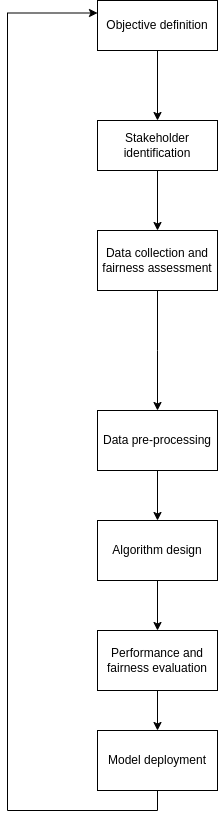
\includegraphics[width=.5\textwidth,height=1\textwidth]{final.png}
    \caption{Fair-by-Design Workflow}
\end{figure}

In the subsequent sections, each of these steps will be comprehensively explored to provide a detailed understanding of the fair-by-design workflow and its ethical underpinnings.

\section{Objective Definition}
\label{section:objective-definition}

The inaugural stage of a fair-by-design workflow mandates the meticulous definition of the system's objectives. The clarity and precision with which these objectives are articulated play a pivotal role in shaping subsequent design decisions. Within the realm of fairness, it becomes imperative to explicitly integrate fairness considerations into the articulated objectives.

In setting the system's goals, a nuanced understanding of the broader ethical landscape becomes foundational. This includes a comprehensive grasp of the potential societal impact, the diverse user base, and the nuanced interplay of ethical considerations within the specific domain of application. The deliberate inclusion of fairness considerations at this early juncture ensures that the pursuit of system objectives aligns seamlessly with the overarching ethical principles, reflecting a commitment to equitable and unbiased outcomes.

By explicitly weaving fairness into the fabric of the defined objectives, the fair-by-design approach underscores its commitment to the proactive anticipation and mitigation of biases. This foundational step lays the groundwork for subsequent design choices, framing the entire development process within an ethical framework that prioritizes fairness and aligns with societal values.

\subsection{Key Considerations}

\begin{enumerate}

    \item \emph{Clarity and Precision:}

        \begin{itemize}

            
            \item \emph{Precision in Objective Definition:} The formulation of specific objectives for the system or process demands clarity and precision to establish a focused and effective approach. This entails articulating goals that are both clear and measurable, aligning seamlessly with the overarching purpose of the system. Objectives should strive to eliminate ambiguity, providing a concrete understanding of the system's intended achievements. 
            
            The significance of clarity in objectives extends beyond the initial definition phase. It serves as a guiding beacon throughout the subsequent development and implementation processes, ensuring a cohesive and purposeful trajectory. Furthermore, the articulation of unambiguous objectives facilitates the accurate evaluation of the system's success in attaining its intended goals. This commitment to precision in objective definition not only enhances the effectiveness of the system but also contributes to a more robust and evaluative framework for assessing its overall impact and success.
            
            \item \emph{Comprehensive Articulation of System Attributes:} A foundational aspect of the fair-by-design workflow involves the explicit and detailed articulation of the system's intended functionalities, goals, and expected outcomes. This comprehensive elucidation is indispensable for fostering a profound understanding of the system or process.

            The delineation of functionalities necessitates a detailed description, outlining the specific tasks or operations the system is designed to execute. Precision in stating goals becomes paramount, emphasizing the overarching aims that the system aspires to achieve. Additionally, the expected outcomes must be clearly defined, specifying the anticipated results or benefits that stakeholders can expect from the successful implementation of the system.
            
            This level of clarity ensures a seamless alignment between development efforts and the envisioned impact, facilitating effective communication and collaboration among all involved parties. By providing a robust framework of understanding, this articulation of functionalities, goals, and outcomes becomes instrumental in guiding subsequent design decisions and ensuring that the fair-by-design approach remains steadfast in its commitment to transparent and equitable system development.        
        
        \end{itemize}
    
    \item \emph{Incorporating Fairness:}

        \begin{itemize}
            
            \item \emph{Explicit Emphasis on Fairness:} A paramount facet in the fair-by-design workflow involves the explicit and emphatic statement of the importance of fairness in achieving the defined objectives. Fairness is not merely an auxiliary consideration; it stands as a foundational principle that underpins the ethical and equitable functioning of the system.

            By explicitly prioritizing fair treatment for all individuals or groups affected by the system, it serves as a cornerstone for enhancing trust, mitigating potential biases, and promoting inclusivity. This acknowledgment of fairness as a non-negotiable element in the pursuit of objectives reflects a resolute commitment to ethical practices and responsible deployment.
            
            Furthermore, positioning fairness as a critical consideration aligns the system with societal values, legal standards, and stakeholder expectations. This alignment not only fosters a positive impact on the system's performance but extends to its broader social implications. The explicit emphasis on fairness within the fair-by-design framework signifies a dedication to cultivating technology that not only meets its functional objectives but does so with a keen awareness of the ethical imperatives that define its relationship with the individuals and communities it serves.
                                    
            \item \emph{Alignment of Fairness with System Purpose:} The seamless alignment of fairness with the overarching purpose of the system is an integral determinant of its effectiveness and societal impact. Fairness ensures that the system operates in a manner characterized by justice, impartiality, and a consideration of diverse perspectives. In this alignment, fairness becomes a cornerstone for enhancing the legitimacy of outcomes, promoting equal opportunities, and guarding against discriminatory practices.

            Incorporating fairness as a core element within the system not only facilitates the ethical attainment of defined objectives but also contributes significantly to cultivating a more inclusive and equitable societal framework. Fairness becomes a driving force that not only strengthens the system's purpose but also fosters trust and positive engagement among users and stakeholders. Simultaneously, it serves as a proactive safeguard, minimizing negative consequences and disparities that may arise from the system's operations.
            
            In essence, the intentional integration of fairness aligns the system with a broader ethical compass, elevating its purpose beyond mere functionality to a realm where societal impact is inherently intertwined with principles of justice, equity, and ethical responsibility.

        \end{itemize}
    
    \item \emph{Balancing Objectives:}

        \begin{itemize}
            
            \item \emph{Balancing Multiple Objectives with Fairness:} Striking a delicate balance among various objectives is paramount, demanding meticulous consideration to prevent the compromise of fairness in the pursuit of other goals. While the system may encompass multifaceted objectives such as efficiency, accuracy, and speed, the commitment to fairness should remain unwavering.

            This delicate equilibrium requires optimizing the system to meet its diverse goals without perpetuating biases or causing harm to specific groups. It necessitates a nuanced approach, where trade-offs are carefully evaluated to ensure that fairness is not sacrificed for the sake of expediency or efficiency. By upholding fairness as a foundational principle, the system can achieve a harmonious equilibrium, fostering an environment where diverse objectives are met without undermining the ethical considerations embedded in the pursuit of those objectives.

            This commitment to balance not only enhances the ethical standing of the system but also contributes to the creation of a technology landscape where fairness is not an afterthought but an integral and non-negotiable aspect of system optimization. In navigating these complexities, the fair-by-design framework becomes a guiding compass, ensuring that the pursuit of efficiency and other objectives remains harmonized with the overarching commitment to fairness.
            
            \item \emph{Identifying Conflicts and Establishing Priorities:} In navigating the intricate landscape of system development, a crucial undertaking involves identifying potential conflicts and establishing priorities among competing objectives. While fairness stands as a paramount consideration, it may at times seem to conflict with other objectives such as efficiency or cost-effectiveness. In such scenarios, conducting a thorough analysis becomes imperative to discern the nature and extent of these conflicts.

            Establishing clear priorities involves a meticulous assessment of the relative importance of each objective and determining where compromises can be made without jeopardizing the ethical principles underpinning fairness. This process demands a careful weighing of trade-offs, with the ultimate goal of aligning competing objectives in a manner that upholds fairness as a non-negotiable priority while still achieving overall system efficiency and effectiveness.
            
            The pursuit of these priorities is not a one-size-fits-all endeavor but requires a nuanced understanding of the specific context and ethical implications. By engaging in this deliberate process of conflict resolution and priority establishment, the fair-by-design workflow ensures that fairness remains at the forefront, serving as a guiding principle that shapes the overall development trajectory of the system.

        \end{itemize}

\end{enumerate}

\subsection{Detailed Implementation Steps}

\subsubsection{Stakeholder Engagement}

\begin{itemize}

    \item \emph{Objective Setting Through Stakeholder Engagement:} The definition of objectives within the fair-by-design workflow is a collaborative and inclusive process that begins by engaging key stakeholders, including end-users, developers, and decision-makers. This fundamental step fosters a collective and participatory approach to system development, where the diverse perspectives and insights of stakeholders are incorporated into the objective-setting process.

    End-users, with their real-world experience, provide valuable input rooted in practical needs. Developers contribute technical expertise, and decision-makers bring strategic considerations to the table. This collective engagement ensures not only a comprehensive understanding of the system's purpose but also enhances the likelihood of creating a solution that aligns with the varied requirements and expectations of all involved parties.

    The collaborative foundation established through stakeholder engagement is essential for achieving consensus on objectives. This consensus, in turn, paves the way for the successful development and implementation of a fair and effective system. By involving stakeholders from the outset, the fair-by-design workflow acknowledges the richness of diverse perspectives, fostering a sense of ownership and collective responsibility in the pursuit of objectives that are both ethically grounded and practically relevant.\item \emph{Objective Setting Through Stakeholder Engagement:} The definition of objectives within the fair-by-design workflow is a collaborative and inclusive process that begins by engaging key stakeholders, including end-users, developers, and decision-makers. This fundamental step fosters a collective and participatory approach to system development, where the diverse perspectives and insights of stakeholders are incorporated into the objective-setting process.

    End-users, with their real-world experience, provide valuable input rooted in practical needs. Developers contribute technical expertise, and decision-makers bring strategic considerations to the table. This collective engagement ensures not only a comprehensive understanding of the system's purpose but also enhances the likelihood of creating a solution that aligns with the varied requirements and expectations of all involved parties.

    The collaborative foundation established through stakeholder engagement is essential for achieving consensus on objectives. This consensus, in turn, paves the way for the successful development and implementation of a fair and effective system. By involving stakeholders from the outset, the fair-by-design workflow acknowledges the richness of diverse perspectives, fostering a sense of ownership and collective responsibility in the pursuit of objectives that are both ethically grounded and practically relevant.
    
    \item \emph{Implementation:}

        \begin{itemize}
            
            \item Conduct stakeholder interviews, surveys, or workshops to gather insights into their expectations and requirements.
            
            \item Ensure diverse representation to capture a comprehensive range of perspectives.
            
            \item Facilitate open discussions to uncover implicit biases or preferences that may influence objectives.
        
        \end{itemize}

\end{itemize}

\subsubsection{Define Performance Metrics}

\begin{itemize}

    \item \emph{Objective:} Specify the metrics that will serve as the yardstick for measuring the success of the system, ensuring a well-defined and quantitative framework for evaluation. These metrics should be meticulously selected to align with the established objectives, encompassing both technical performance and fairness considerations.

    For technical aspects, metrics such as accuracy, precision, recall, and F1 score may be relevant, providing insights into the system's overall effectiveness. Simultaneously, metrics specifically designed to assess fairness, such as disparate impact, equalized odds, and overall fairness indices, should be included to gauge the system's fairness.
    
    The chosen metrics must accurately reflect the intended outcomes and contribute to a comprehensive assessment, enabling a nuanced understanding of the system's success. Upholding fairness as a paramount criterion, the fair-by-design approach ensures that the selected metrics go beyond traditional performance indicators, providing a holistic evaluation that considers both technical proficiency and ethical considerations. This commitment to a diverse set of metrics facilitates a comprehensive understanding of the system's impact, fostering an environment where success is measured not only by technical prowess but also by the ethical principles embedded in the fair-by-design framework.    
    
    \item \emph{Implementation:}
        
    \begin{itemize}
            
        \item Identify traditional performance metrics (e.g., accuracy, precision, recall) relevant to the system's goals.
            
        \item Integrate fairness-specific metrics, such as disparate impact, equalized odds, or statistical parity, depending on the context.
            
        \item Establish a comprehensive set of metrics that collectively address both general system performance and fairness considerations.

    \end{itemize}

\end{itemize}

\subsubsection{Ethical Considerations}

\begin{itemize}

    \item \emph{Objective:} Undertake a comprehensive exploration of the ethical implications associated with the defined objectives, conducting a thorough examination to anticipate and address potential ethical challenges. This involves a deep dive into how the system's goals and functionalities may intersect with broader ethical considerations, including privacy, security, and societal impact.

    Consider the implications for different stakeholder groups, ensuring that the system's objectives align with ethical standards and societal values. This involves a proactive approach, articulating clear guidelines and safeguards to mitigate ethical concerns, thereby promoting transparency and accountability throughout the development and implementation phases.
    
    By proactively addressing ethical implications, the system positions itself to navigate complex ethical landscapes responsibly. This commitment to ethical foresight not only upholds ethical considerations alongside technical functionalities but also contributes to the creation of a technology-driven environment that prioritizes ethical principles. Through this conscientious approach, the fair-by-design workflow not only aims for technical excellence but also seeks to embed a strong ethical foundation, fostering a system that is not only proficient but also ethically responsible.

    \item \emph{Implementation:}

        \begin{itemize}

            \item Conduct an ethical impact assessment to identify potential biases or unintended consequences.

            \item Evaluate the ethical implications of each performance metric, ensuring alignment with fairness goals.

            \item Anticipate scenarios where ethical dilemmas may arise and establish guidelines for resolution.

        \end{itemize}

\end{itemize}

\subsubsection{Documentation}

\begin{itemize}

    \item \emph{Objective:} Rigorously document the defined objectives in a clear and comprehensive manner, ensuring that each objective is articulated with precision and detail. Provide a detailed overview of the intended functionalities, goals, and expected outcomes, leaving no room for ambiguity.

    Utilize concise and unambiguous language to capture the essence of each objective, outlining the specific tasks or functionalities the system aims to achieve. Include any relevant context or background information that enhances the understanding of each objective. This documentation serves as a foundational reference for all stakeholders involved in the development and implementation of the system.

    The goal is to foster a shared understanding of the project's overarching goals and guiding principles among team members, end-users, and decision-makers throughout the system's lifecycle. Clarity and comprehensiveness in objective documentation are indispensable for effective communication and collaboration. By meticulously documenting the objectives, the fair-by-design workflow not only ensures alignment with ethical principles but also establishes a robust foundation for informed decision-making and collective engagement across all stages of system development.
    
    \item \emph{Implementation:}

        \begin{itemize}

            \item Create a detailed objective statement that serves as a reference point for all stakeholders.

            \item Document the rationale behind the inclusion of fairness considerations in the objectives.

            \item Maintain a living document that can be updated as objectives evolve or new insights emerge.

        \end{itemize}

\end{itemize}

\subsection{Significance}

Defining objectives with precision, incorporating fairness considerations, and establishing clear performance metrics are the foundational pillars of a fair-by-design approach. Precision in objective definition is crucial to avoid ambiguity and guide the development process effectively. Integrating fairness considerations from the outset ensures that ethical principles are not an afterthought but integral to the system's purpose. Clear performance metrics enable the systematic evaluation of the system's success and adherence to fairness goals.

Together, these steps create a comprehensive framework that not only aligns the system with ethical standards but also meets stakeholder expectations, fostering trust and accountability throughout the development lifecycle. This approach not only enhances the effectiveness of the system but also contributes to a technology landscape where ethical considerations are seamlessly woven into the fabric of technological advancements. Through a meticulous and proactive fair-by-design methodology, the system becomes not just a product of technical prowess but a testament to ethical responsibility and societal relevance.

\section{Stakeholder Identification}
\label{section:stakeholder-identification}

Engaging key stakeholders is a foundational step in shaping the objectives of a fair-by-design workflow. Stakeholders, representing diverse perspectives and interests, bring invaluable insights that contribute to defining the system's purpose. Involving a range of stakeholders ensures a comprehensive understanding of ethical implications and societal expectations. This inclusive approach not only fosters a sense of collective responsibility but also helps in addressing potential biases and concerns early in the design process.

By incorporating various viewpoints, the fair-by-design workflow becomes more attuned to the needs of different communities and stakeholders, enhancing the overall fairness and effectiveness of the system. This collaborative engagement not only contributes to the ethical grounding of the system but also establishes a sense of shared ownership and accountability among stakeholders. Through this inclusive approach, the fair-by-design methodology ensures that the development process is enriched by a diversity of perspectives, making the resulting system more responsive, transparent, and aligned with the values and expectations of the broader community it serves.

\subsection{Key Considerations}

\begin{enumerate}

    \item \emph{Diverse Representation:}

        \begin{itemize}

            \item \emph{Ensuring Inclusive Stakeholder Representation:} In the fair-by-design approach, ensuring the inclusion of stakeholders who represent a diverse range of perspectives is paramount. This encompasses stakeholders such as end-users, developers, decision-makers, and members of affected communities. Each stakeholder group contributes unique insights and experiences that are crucial for shaping a system that is equitable and aligned with ethical principles.

            End-users provide practical insights into how the system will be experienced, developers offer technical expertise, decision-makers provide strategic guidance, and affected communities bring perspectives on potential societal impacts. By actively involving this diverse set of stakeholders, the fair-by-design workflow gains a more holistic understanding of potential biases, ethical considerations, and the broader societal context, ultimately leading to a more inclusive and equitable outcome.
            
            This intentional inclusion of diverse voices not only enhances the fairness of the system but also establishes a collaborative foundation that reflects a commitment to responsible and ethical AI development. The fair-by-design methodology recognizes the significance of varied perspectives in creating technology that not only functions effectively but also considers the diverse needs and impacts on the communities it serves.

        \end{itemize}
    
    \item \emph{Inclusive Decision-Making:}
        
    \begin{itemize}
    
        \item \emph{Fostering Inclusive Decision-Making:} Fostering an inclusive environment is integral to the fair-by-design approach, ensuring that stakeholders actively participate in decision-making processes related to the system's objectives. This inclusivity encourages diverse perspectives, fostering a collaborative atmosphere where each stakeholder's input is valued.

        Establishing open channels of communication and providing opportunities for meaningful engagement empowers stakeholders to contribute their insights effectively. By creating an inclusive space, the fair-by-design workflow not only captures a broader range of perspectives but also cultivates a sense of ownership among stakeholders. This collaborative decision-making process enhances transparency, builds trust, and ultimately results in a system that is more responsive to the needs and values of the varied stakeholders involved.
        
        Through active and inclusive participation, stakeholders become co-creators of the system, contributing to its development in a manner that reflects a shared commitment to fairness and ethical considerations. This inclusive decision-making not only strengthens the ethical foundation of the system but also fosters a collaborative culture that extends beyond the development phase, influencing the ongoing relationship between the technology and the diverse communities it serves.

    \end{itemize}
    
    \item \emph{Transparent Communication:}
    
    \begin{itemize}

        \item \emph{Maintaining Transparent Communication Channels:} In the fair-by-design approach, maintaining transparent communication channels is crucial to keeping stakeholders informed about the development process and gathering their input effectively. Transparent communication fosters trust and ensures that stakeholders are aware of the system's progress, objectives, and any potential implications.

        Regular updates, clear documentation, and accessible information contribute to an open dialogue, allowing stakeholders to stay engaged and provide valuable feedback. This proactive approach to communication not only enhances the collaborative decision-making process but also promotes a shared understanding of the ethical considerations embedded in the system.
        
        Transparent communication channels serve as a cornerstone of the fair-by-design workflow, fostering a sense of inclusivity and shared responsibility among all stakeholders involved. By keeping the lines of communication open, the fair-by-design methodology not only embraces diverse perspectives but also actively engages stakeholders in a continuous dialogue that extends throughout the system's lifecycle. This commitment to transparency is instrumental in building and sustaining trust, creating an environment where stakeholders feel empowered and informed in their roles as contributors to the ethical development of the technology.

    \end{itemize}

\end{enumerate}

\subsection{Detailed Implementation Steps}

\subsubsection{Stakeholder Mapping}

\begin{itemize}
    
    \item \emph{Objective:} Identifying and mapping key stakeholders is a crucial step in the fair-by-design approach to understand and incorporate diverse perspectives in the system's development. Key stakeholders include end-users, developers, decision-makers, and affected communities, each bringing unique insights and interests to the table.

    End-users provide valuable feedback based on their experiences and expectations, guiding user-centric design. Developers contribute technical expertise, ensuring the feasibility and efficiency of the system. Decision-makers offer strategic input aligning the system with broader organizational goals. Affected communities bring a contextual understanding of societal impacts, helping navigate ethical considerations.
    
    By mapping these stakeholders, the fair-by-design workflow ensures a holistic and inclusive approach, considering the varied interests and perspectives that shape the system's objectives and ethical considerations. This intentional identification and mapping process set the foundation for a collaborative and well-informed decision-making process, where the diverse voices of stakeholders are actively incorporated into the development trajectory of the system.

    \item \emph{Implementation:}
    
    \begin{itemize}
    
        \item Create a stakeholder map that identifies different stakeholder groups and their respective roles and interests.
    
        \item Prioritize stakeholders based on their influence on or impact from the system.
    
    \end{itemize}

\end{itemize}

\subsubsection{Engagement Strategies}

\begin{itemize}

    \item \emph{Objective:} Developing effective strategies for stakeholder engagement in the objective-setting process is pivotal for a fair-by-design workflow. Begin by conducting stakeholder analysis to identify key individuals and groups. Establish clear communication channels to disseminate information and gather feedback. Organize workshops, focus groups, or collaborative sessions to facilitate active participation. Tailor engagement methods to suit diverse stakeholders, ensuring inclusivity.

    Provide accessible documentation outlining the proposed objectives and ethical considerations. Emphasize the value of each stakeholder's input and foster an open dialogue to address concerns. Regularly update stakeholders on the progress, incorporating their feedback iteratively.
    
    By employing these strategies, a fair-by-design workflow ensures comprehensive engagement, enriching the objective-setting process with diverse perspectives and reinforcing ethical considerations. This proactive and inclusive approach to stakeholder engagement not only enhances the quality of the objectives but also contributes to a collaborative and transparent development process, where stakeholders feel valued and actively contribute to the ethical foundation of the system.

    \item \emph{Implementation:}

    \begin{itemize}

        \item Tailor engagement strategies to the characteristics of each stakeholder group (e.g., workshops, surveys, focus groups).

        \item Clearly communicate the importance of their input in shaping the ethical foundations of the system.

    \end{itemize}

\end{itemize}

\subsubsection{Inclusive Workshops or Meetings}

\begin{itemize}

    \item \emph{Objective:} In fostering an inclusive fair-by-design approach, organizing workshops or meetings is instrumental for stakeholder engagement in defining objectives. These sessions provide a platform for active participation, allowing diverse stakeholders, including end-users, developers, decision-makers, and affected communities, to contribute insights.

    The workshops should be designed to encourage open dialogue, ensuring that each perspective is heard and considered. Employ facilitation techniques that promote inclusivity, such as structured discussions, brainstorming sessions, or collaborative activities. By facilitating these inclusive workshops, the fair-by-design workflow embraces diverse viewpoints, enriching the objective-setting process and reinforcing its commitment to ethical considerations.
    
    Through these workshops, the fair-by-design methodology actively encourages a collaborative environment where stakeholders feel empowered to contribute, fostering a sense of ownership and shared responsibility in shaping the system's objectives. This inclusive approach not only enhances the quality of the objectives but also establishes a foundation for continued collaboration and engagement throughout the development lifecycle.

    \item \emph{Implementation:}

    \begin{itemize}

        \item Organize collaborative sessions that encourage open dialogue and the exchange of diverse perspectives.

        \item Provide a platform for stakeholders to express their values, concerns, and expectations related to fairness in the system.

    \end{itemize}

\end{itemize}

\subsubsection{Feedback Collection}

\begin{itemize}

    \item \emph{Objective:} After defining initial objectives and ethical considerations in the fair-by-design workflow, it is crucial to gather feedback from stakeholders. Establish a feedback loop through surveys, interviews, or focus group discussions to ensure that the proposed objectives resonate with the diverse perspectives of stakeholders. This iterative process allows for refinements and adjustments based on the input received.

    Actively seeking feedback fosters collaboration and ensures that the fair-by-design approach remains responsive to the evolving needs and expectations of stakeholders throughout the system's development. This ongoing feedback loop not only contributes to the iterative improvement of objectives but also reinforces a culture of continuous engagement, where stakeholders play an active role in shaping the ethical foundation of the technology.

    \item \emph{Implementation:}

    \begin{itemize}

        \item Utilize surveys, interviews, or online platforms to collect structured feedback.

        \item Encourage stakeholders to provide qualitative insights that may not be captured by quantitative methods.

    \end{itemize}

\end{itemize}

\subsection{Significance}

Stakeholder identification is a pivotal aspect of ensuring the fair and inclusive development of a system. Involving stakeholders from diverse backgrounds and perspectives allows the ethical considerations embedded in the objectives to more accurately reflect the values and expectations of the broader community. By recognizing and engaging with a variety of stakeholders, including end-users, developers, decision-makers, and representatives from affected communities, the fair-by-design approach becomes more comprehensive and responsive to the multifaceted needs and concerns of the people who will interact with or be impacted by the system.

This inclusive process contributes to the development of a system that is not only technically sound but also ethically grounded and considerate of various societal perspectives. The intentional involvement of diverse stakeholders ensures that the resulting technology aligns with ethical standards and is more likely to meet the expectations of the communities it serves, fostering a sense of trust and accountability in the development process.


%----------------------------------------------------------------------------------------
\chapter{Validation} % possible chapter for Projects
\label{chap:validation}
%----------------------------------------------------------------------------------------

Since every algorithm choice in the algorithm design step of the workflow required pre-trained estimator, 3 estimators have been choice to have a comprehensive evaluation of the performance of the workflow proposed here.

\section{Experiment setup}

For each of the previous approaches have been chosen 3 models to perform the prediction:

\begin{enumerate}

    \item \text{RandomForest Classifier}: RandomForest Classifier is a popular machine learning algorithm that leverages an ensemble of decision trees to make predictions. It excels at tasks like classification and regression, offering robustness against overfitting and high accuracy by aggregating the predictions of multiple decision trees. It's a versatile tool used in various applications, from finance to healthcare and image analysis.
    
    \item \textbf{LGB Classifier}: LightGBM, short for Light Gradient Boosting Machine, stands out as a powerful gradient boosting framework that originated from the innovation labs at Microsoft. Engineered with a specific focus on efficiency, speed, and scalability, LightGBM has become a prominent choice in the realm of machine learning, demonstrating exceptional performance across various tasks.
    
    \item \textbf{DecisionTree Classifier}: DecisionTree Classifier is a specific type of machine learning algorithm primarily used for classification tasks. It constructs a tree-like model, where each internal node represents a decision based on a specific feature, and each leaf node denotes the predicted class label for the input data point.

\end{enumerate}

On the previous models is applied the GridSearch with a \emph{cv} of 10 in order to select the best parameters combination for each one. In the following are reported the specific parameters for each model:

\begin{enumerate}
    
    \item RandomForest Classifier:
    
    \begin{enumerate}
       
        \item \emph{n\textunderscore estimators}: [10, 100, 10]
       
        \item \emph{criterion}: [gini, entropy, log\textunderscore loss]
       
        \item \emph{max\textunderscore depth}: [10, 50, 10]
       
        \item \emph{max\textunderscore leaf\textunderscore nodes}: [10, 50, 10]
    
    \end{enumerate}
    
    \item LGB Classifier:
    
    \begin{enumerate}

        \item \emph{C}: [0.1, 1, 10]

        \item \emph{kernel}: ['linear', 'rbf', 'poly']

        \item \emph{gamma}: [0.5, 1, 1.5, 2.5]

    \end{enumerate}
    
    \item DecisionTree Classifier:
    
    \begin{enumerate}
    
        \item \emph{criterion}: [gini, entropy, log\textunderscore loss]
    
        \item \emph{max\textunderscore depth}: [10, 50, 10]
    
        \item \emph{max\textunderscore leaf\textunderscore nodes}: [10, 50, 10]
    
    
    \end{enumerate}

\end{enumerate}

Each machine learning model in our study is trained using a training dataset comprising 67\% of the original data, with the remaining 33\% reserved for testing purposes. To provide a more granular analysis, we've segmented the data based on the students' grade levels. Let \( G3 \) represent the subset of the original dataset filtered to include only students enrolled in grade 3.

For the grade 3 dataset (\( G3 \)), the outcomes for every model are presented. Specifically, are highlighted the best-performing model identified during our evaluation process and report its accuracy on the corresponding test set.

This focused analysis on grade 3 allows us to uncover insights that are specific to this grade level. Beyond the accuracy, for each algorithm chosen in the workflow it's performed a fairness evaluation on the results in order to assess the trade-off and the relationship between accuracy and fairness.

\subsection{Performance and fairness evaluation for the Workflow applied with the Fairness through data rebalancing algorithm}

\subsubsection{Best models}

\begin{tabular}{|c|c|}
    \hline
    \textbf{Model} & \textbf{Best parameters} \\
    \hline
    RandomForest Classifier  &  \\
    \hline
    LGB Classifier & \\
    \hline
    DecisionTree Classifier & \\
    \hline
\end{tabular}

\subsubsection{Accuracy}

\begin{tabular}{|c|c|}
    \hline
    \textbf{Model} & \textbf{Accuracy} \\ 
    \hline
    RandomForest Classifier  &  \\
    \hline
    LGB Classifier & \\
    \hline
    DecisionTree Classifier & \\ 
    \hline
\end{tabular}

\subsection{Fairness evaluation}

\begin{tabular}{|c|c|c|}
    \hline
    \textbf{Model} & \textbf{Demographic parity ratio} & \textbf{Equalized odds ratio} \\
    \hline
    RandomForest Classifier & & \\
    \hline
    LGB Classifier & & \\
    \hline
    DecisionTree Classifier & & \\
    \hline
\end{tabular}

\subsection{Performance and fairness evaluation for the Workflow applied with the Fairness through Equalized-Odds Post-Processing with Threshold Optimizer}

\subsubsection{Best models}

\begin{tabular}{|c|c|}
    \hline
    \textbf{Model} & \textbf{Best parameters} \\
    \hline
    RandomForest Classifier  &  \\
    \hline
    LGB Classifier & \\
    \hline
    DecisionTree Classifier & \\
    \hline
\end{tabular}

\subsubsection{Accuracy}

\begin{tabular}{|c|c|}
    \hline
    \textbf{Model} & \textbf{Accuracy} \\ 
    \hline
    RandomForest Classifier  &  \\
    \hline
    LGB Classifier & \\
    \hline
    DecisionTree Classifier & \\ 
    \hline
\end{tabular}

\subsection{Fairness evaluation}

\begin{tabular}{|c|c|c|}
    \hline
    \textbf{Model} & \textbf{Demographic parity ratio} & \textbf{Equalized odds ratio} \\
    \hline
    RandomForest Classifier & & \\
    \hline
    LGB Classifier & & \\
    \hline
    DecisionTree Classifier & & \\
    \hline
\end{tabular}

\subsection{Performance and fairness evaluation for the Workflow applied with the Fairness through GridSearch Reduction algorithm}

\subsubsection{Best models}

\begin{tabular}{|c|c|}
    \hline
    \textbf{Model} & \textbf{Best parameters} \\
    \hline
    RandomForest Classifier  &  \\
    \hline
    LGB Classifier & \\
    \hline
    DecisionTree Classifier & \\
    \hline
\end{tabular}

\subsubsection{Accuracy}

\begin{tabular}{|c|c|}
    \hline
    \textbf{Model} & \textbf{Accuracy} \\ 
    \hline
    RandomForest Classifier  &  \\
    \hline
    LGB Classifier & \\
    \hline
    DecisionTree Classifier & \\ 
    \hline
\end{tabular}

\subsection{Fairness evaluation}

\begin{tabular}{|c|c|c|}
    \hline
    \textbf{Model} & \textbf{Demographic parity ratio} & \textbf{Equalized odds ratio} \\
    \hline
    RandomForest Classifier & & \\
    \hline
    LGB Classifier & & \\
    \hline
    DecisionTree Classifier & & \\
    \hline
\end{tabular}

\subsection{Results comparaison}

%----------------------------------------------------------------------------------------
\chapter{Conclusion}
\label{chap:conclusions}
%----------------------------------------------------------------------------------------

Write conclusions here.


%----------------------------------------------------------------------------------------
% BIBLIOGRAPHY
%----------------------------------------------------------------------------------------

\backmatter

%\nocite{*} % comment this to only show the referenced entries from the .bib file

\bibliographystyle{alpha}
\bibliography{bibliography}


\end{document}